\documentclass{beamer}
\usepackage{relsize}
\usepackage{color}

\usepackage{listings}
\usetheme{CambridgeUS}
%\usepackage{beamerthemesplit} % new 
\usepackage{enumitem}
\usepackage{amsmath}                    % See geometry.pdf to learn the layout options. 
\usepackage{amsthm}                   % See geometry.pdf to learn the layout options. There 
\usepackage{amssymb}                    % See geometry.pdf to learn the layout options. 
\usepackage[utf8]{inputenc} 
\usepackage{graphicx}
\usepackage[english,bulgarian]{babel}

\lstset{language=C++,
                basicstyle=\ttfamily,
                keywordstyle=\color{blue}\ttfamily,
                stringstyle=\color{red}\ttfamily,
                commentstyle=\color{green}\ttfamily,
                morecomment=[l][\color{magenta}]{\#}
}

\newtheorem{mydef}{Дефиниция}[section]
\newtheorem{lem}{Лема}[section]
\newtheorem{thm}{Твърдение}[section]

\DeclareMathOperator{\restrict}{\upharpoonright}

\setitemize{label=\usebeamerfont*{itemize item}%
  \usebeamercolor[fg]{itemize item}
  \usebeamertemplate{itemize item}}

\setbeamercovered{transparent}



\begin{document}
\title[Структури от данни и програмиране]{Дървета} 
\author{Калин Георгиев} 
\frame{\titlepage} 

\section{Интуиция} 


\begin{frame}
\centerline{Интуиция. Йерархична структура от данни}
\end{frame}


\begin{frame}[fragile]
\frametitle{Фамилно дърво}

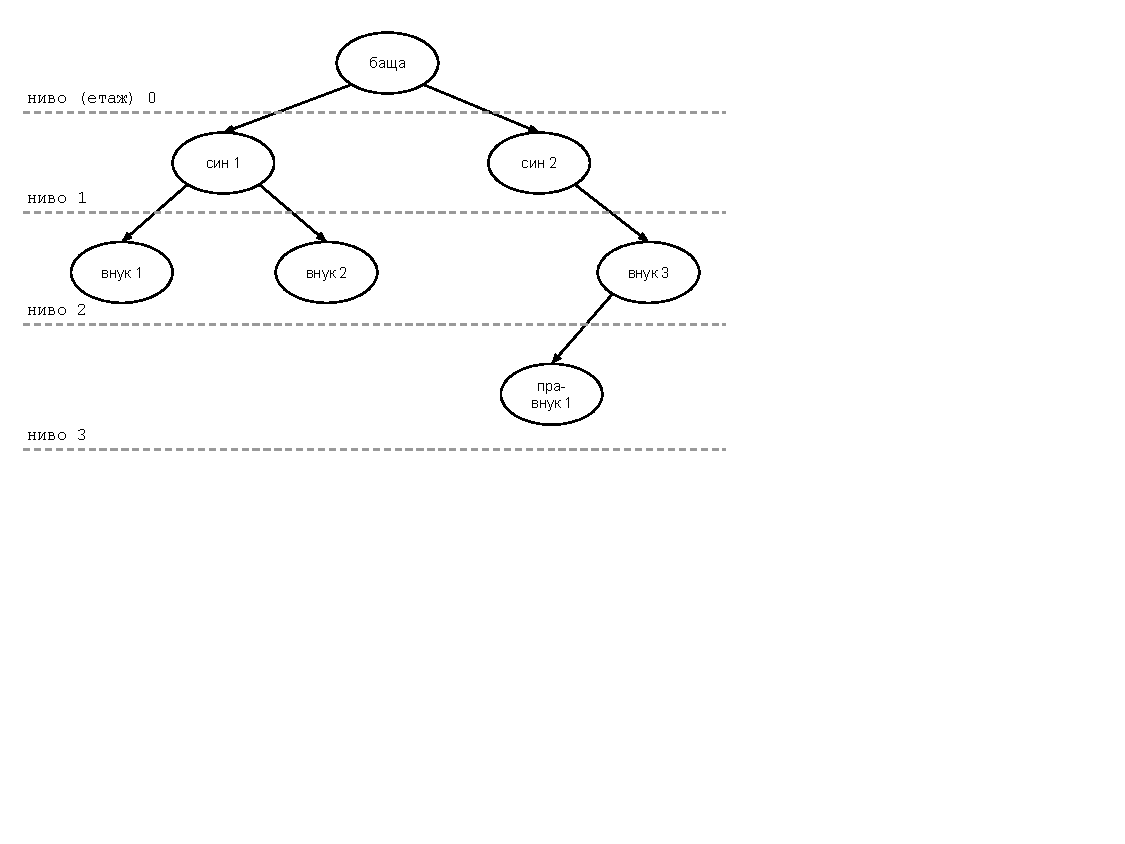
\includegraphics[width=17cm]{images/tree_family_tree}

\end{frame}

\begin{frame}[fragile]
\frametitle{Фамилно дърво}

\begin{columns}[t]
  \begin{column}{0.35\textwidth}

    \begin{itemize}
      \item родител, наследник
      \item корен
      \item листо 
      \item път
      \item ниво
    \end{itemize}

  \end{column}
  \begin{column}{0.65\textwidth}

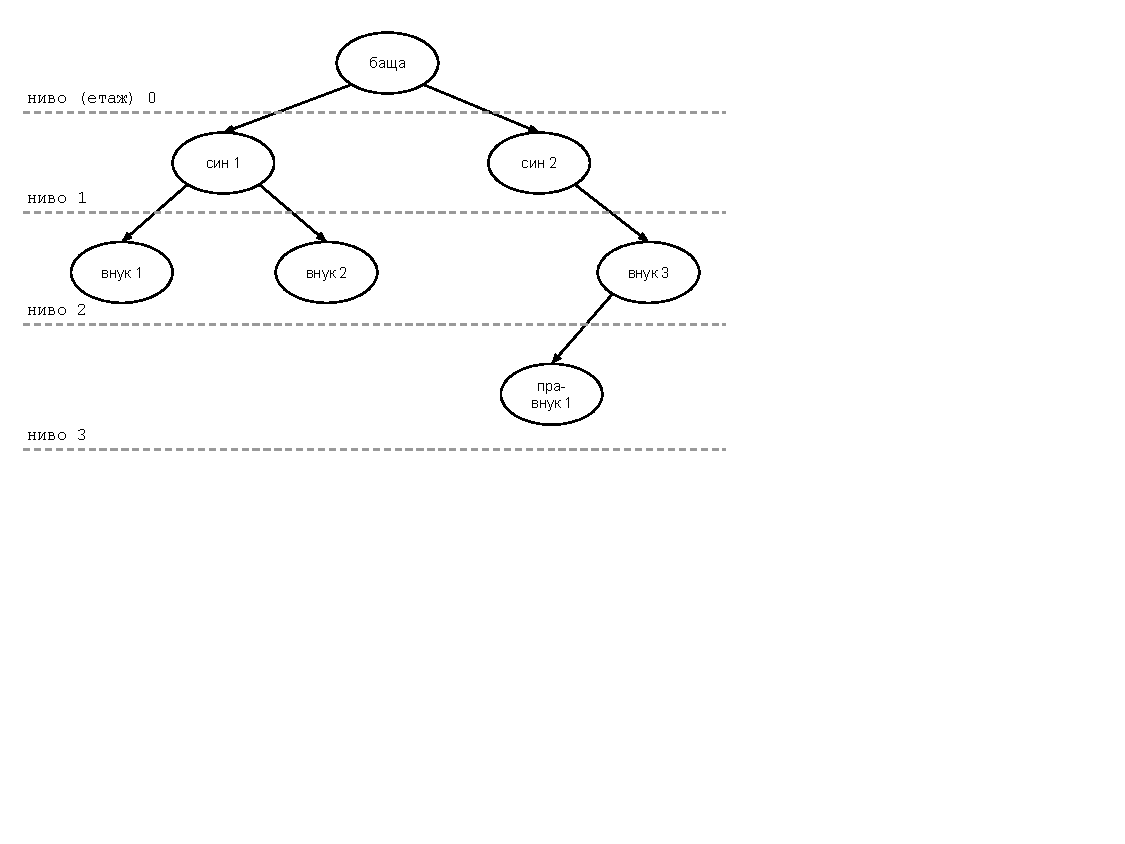
\includegraphics[width=10cm]{images/tree_family_tree}

  \end{column}
\end{columns}

\end{frame}


\begin{frame}[fragile]
\frametitle{Decision Tree}

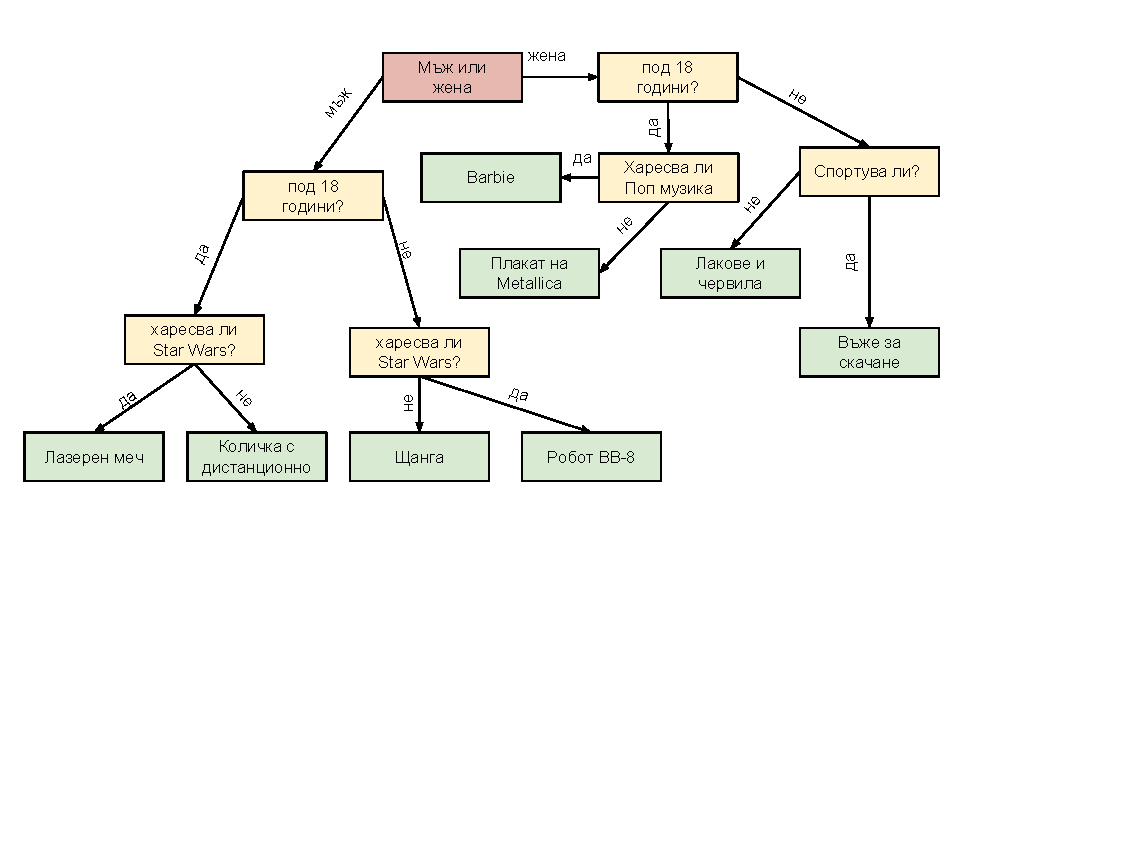
\includegraphics[width=14cm]{images/tree_decision}

\end{frame}

\begin{frame}
\centerline{Формална дефиниция и абстракция}
\end{frame}


\section{Дефиниция} 


\begin{frame}[fragile]
\frametitle{Дефиниции}

    \begin{itemize}
      \item Свързан неориентиран граф без цикли 
    \end{itemize}

    \vspace{1.5em}
     Индуктивна дефиниция

\begin{columns}[t]
  \begin{column}{0.65\textwidth}


    \begin{itemize}
      \item Фиксираме елемент $() \notin D$ и го наричаме \emph{``празно дърво''}
      \item Празното дърво е дърво 
      \item Ако $L_T$ и $R_T$ са дървета, а $x$ е елемент ($x \in D$), то \emph{тройката (структурата)} $T=(x,L_T,R_T)$ наричаме двоично дърво $T$ с \emph{корен} $x$, ляво поддърво $L_T$ и дясно поддърво $R_T$.
    \end{itemize}

  \end{column}
  \begin{column}{0.35\textwidth}

    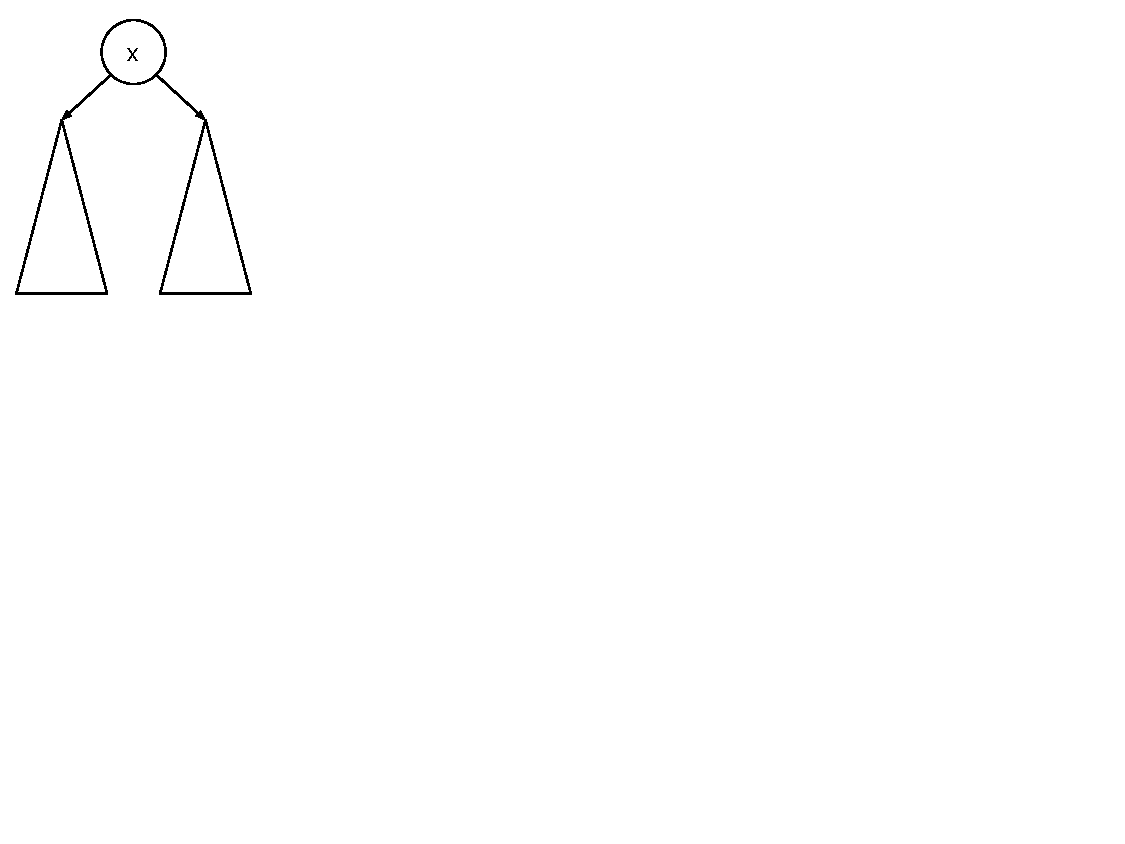
\includegraphics[width=9cm]{images/tree_recursive}

  \end{column}
\end{columns}


\end{frame}



\begin{frame}[fragile]
\frametitle{Дърво с числа}

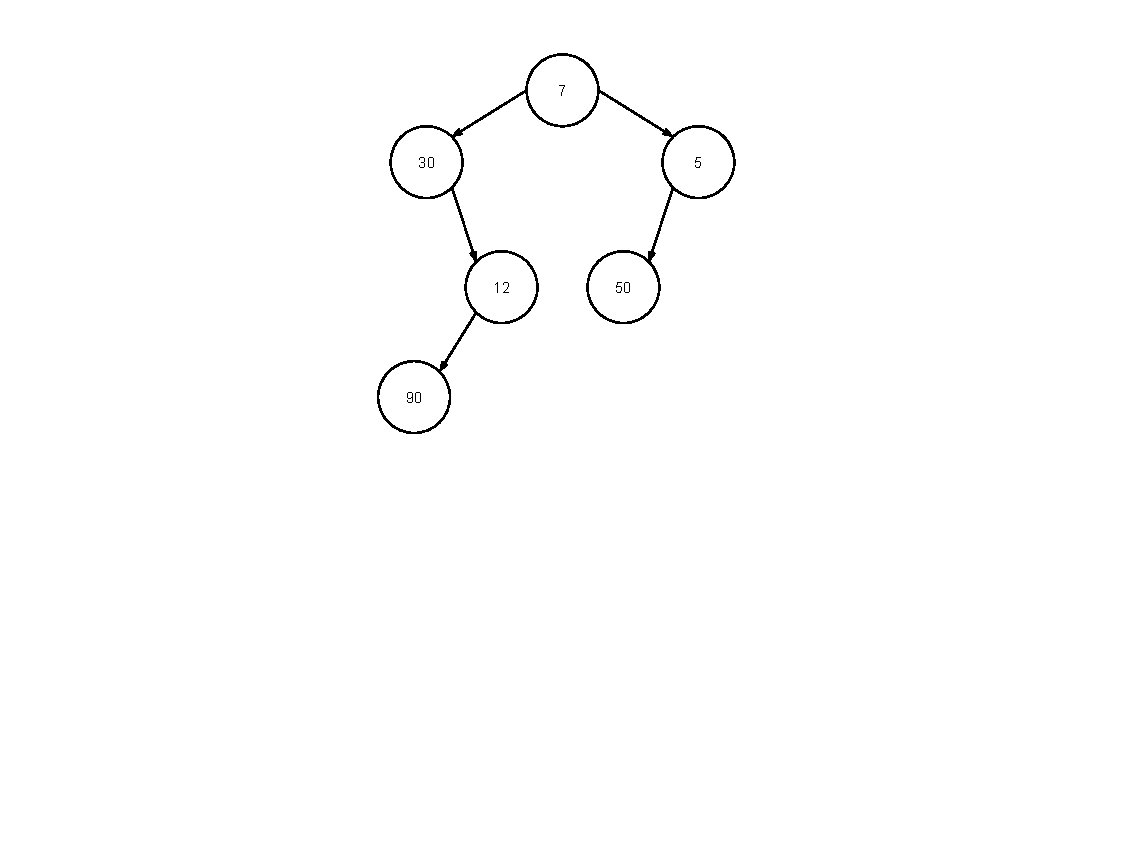
\includegraphics[width=14cm]{images/tree_arbitrary}

\end{frame}


\begin{frame}[fragile]
\frametitle{Двоично наредено дърво}

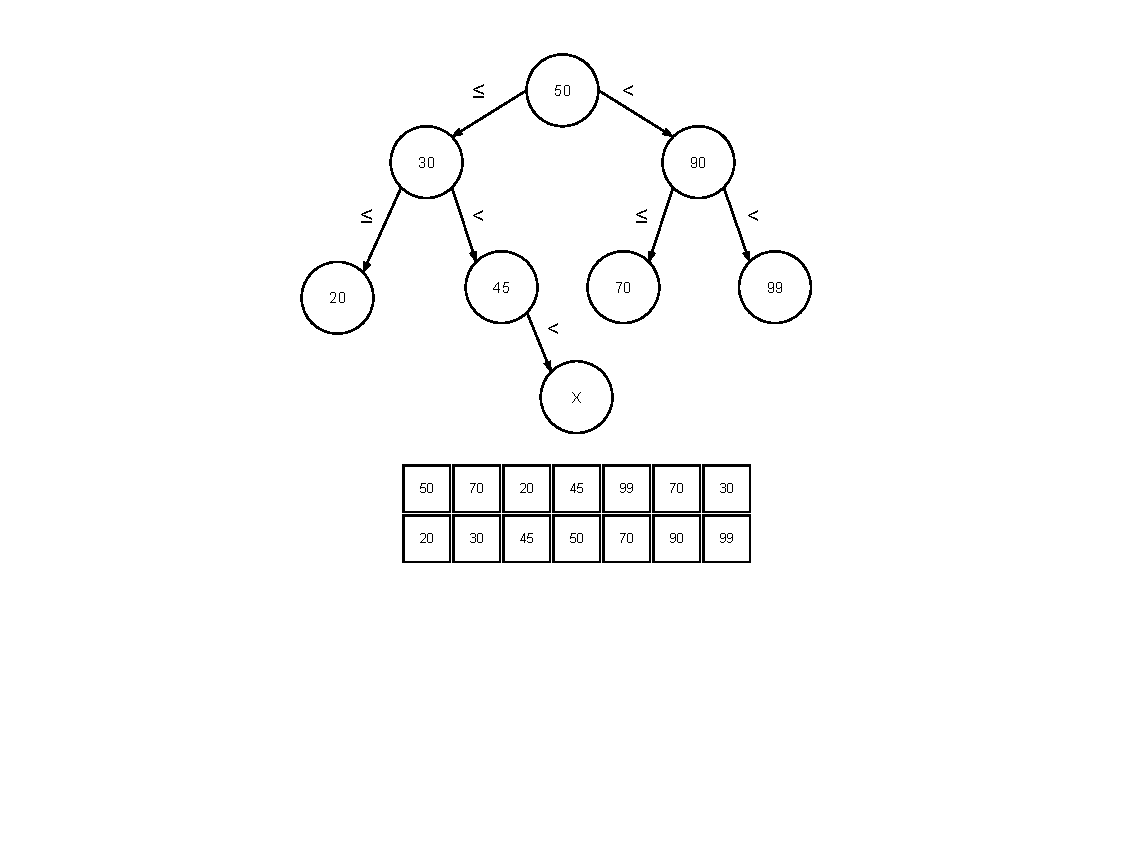
\includegraphics[width=14cm]{images/tree_bot}

\end{frame}

\section{Представяне и операции} 


\begin{frame}
\centerline{Представяне}
\end{frame}


\begin{frame}[fragile]
\frametitle{``Тройна кутия''}

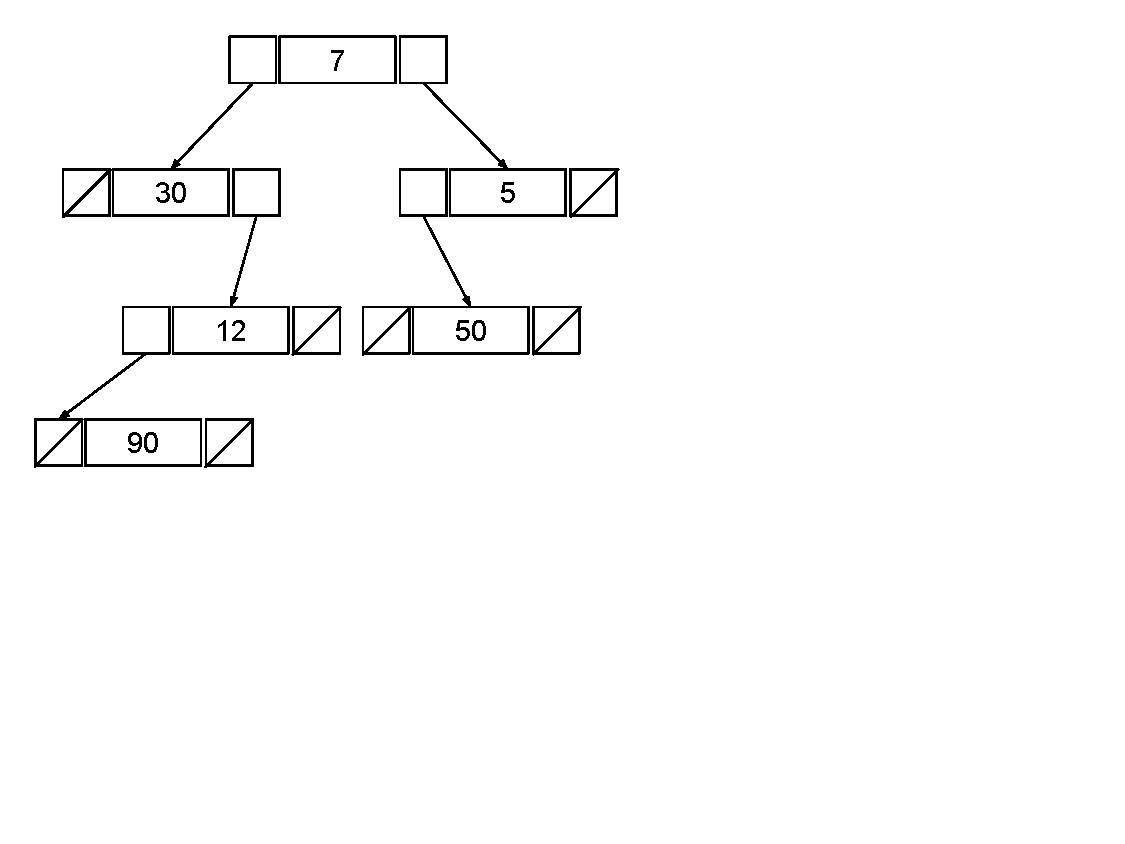
\includegraphics[width=14cm]{images/tree_in_memory}

\end{frame}


\begin{frame}
\centerline{Операции}
\end{frame}

\begin{frame}[fragile]
\frametitle{Добавяне на елемент}

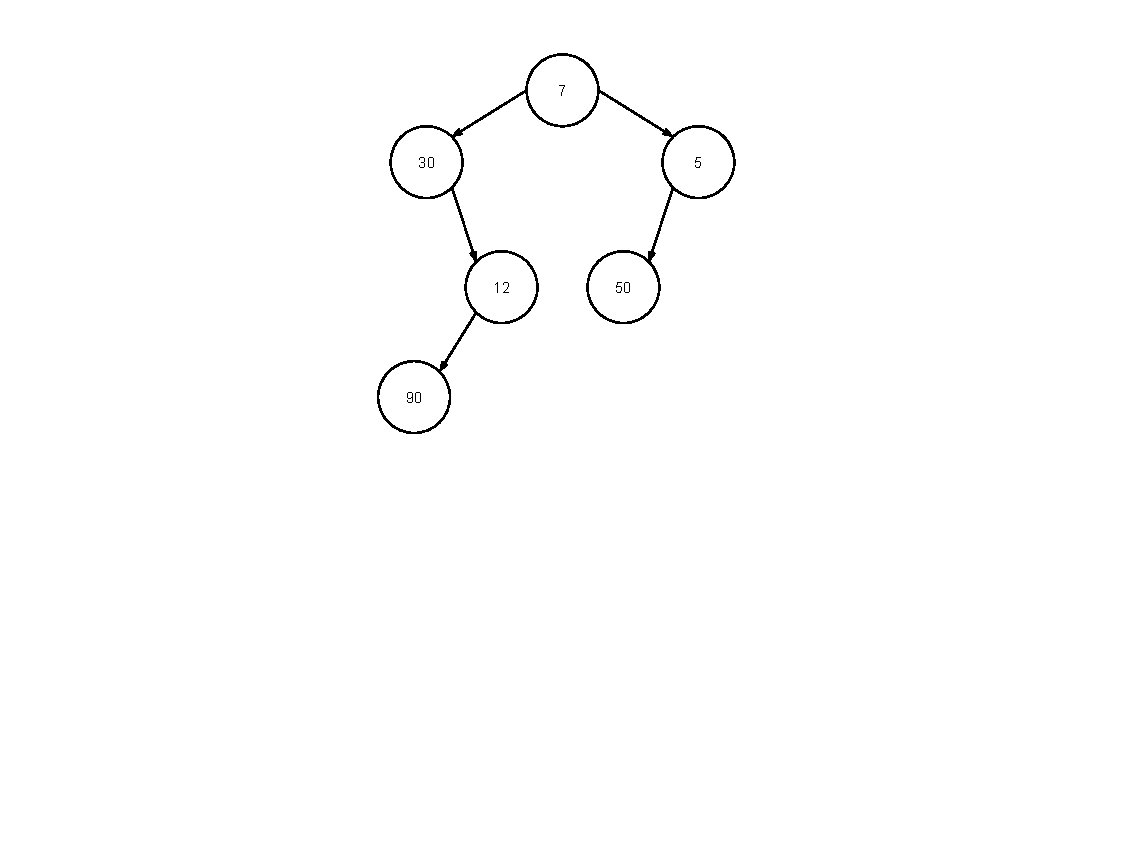
\includegraphics[width=14cm]{images/tree_arbitrary}

\end{frame}


\begin{frame}[fragile]
\frametitle{Следа. Добавяне и намиране на елемент}

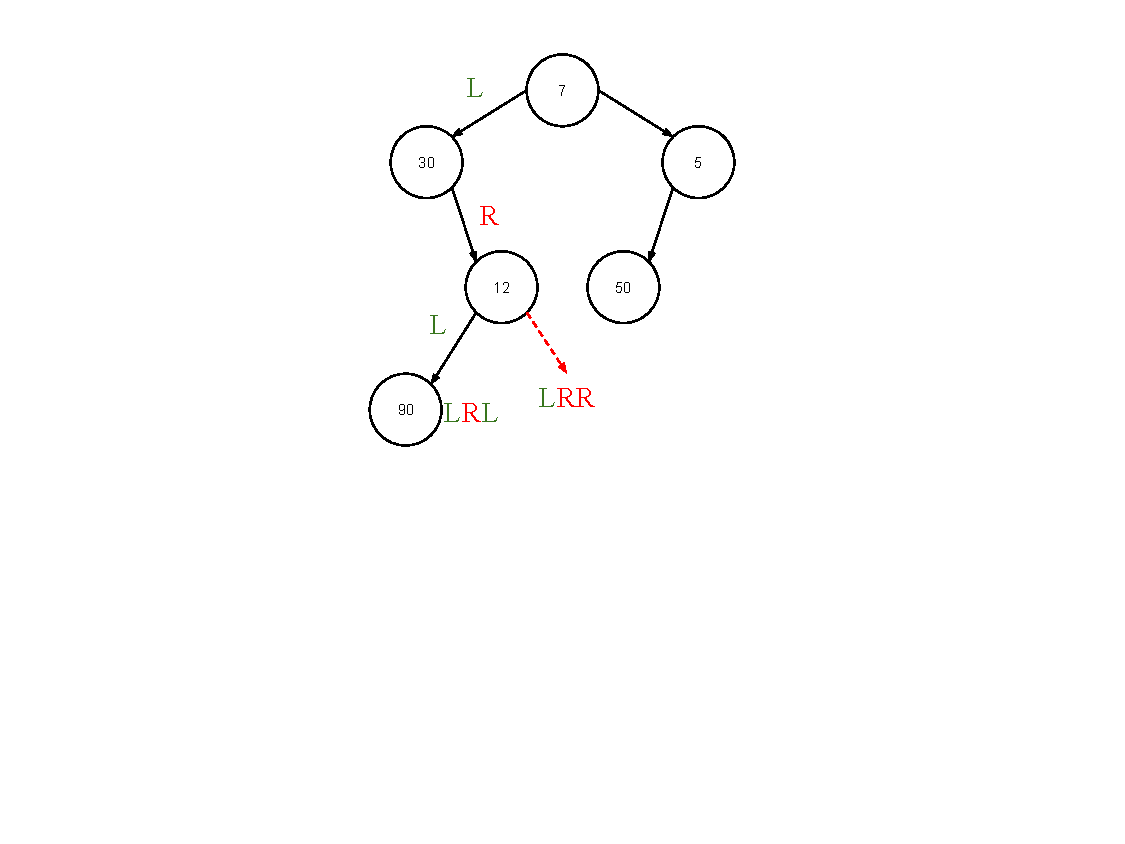
\includegraphics[width=14cm]{images/tree_traces}

\end{frame}


\begin{frame}
\centerline{Рекурсивни операции}
\end{frame}


\begin{frame}[fragile]
\frametitle{Търсене на елемент}

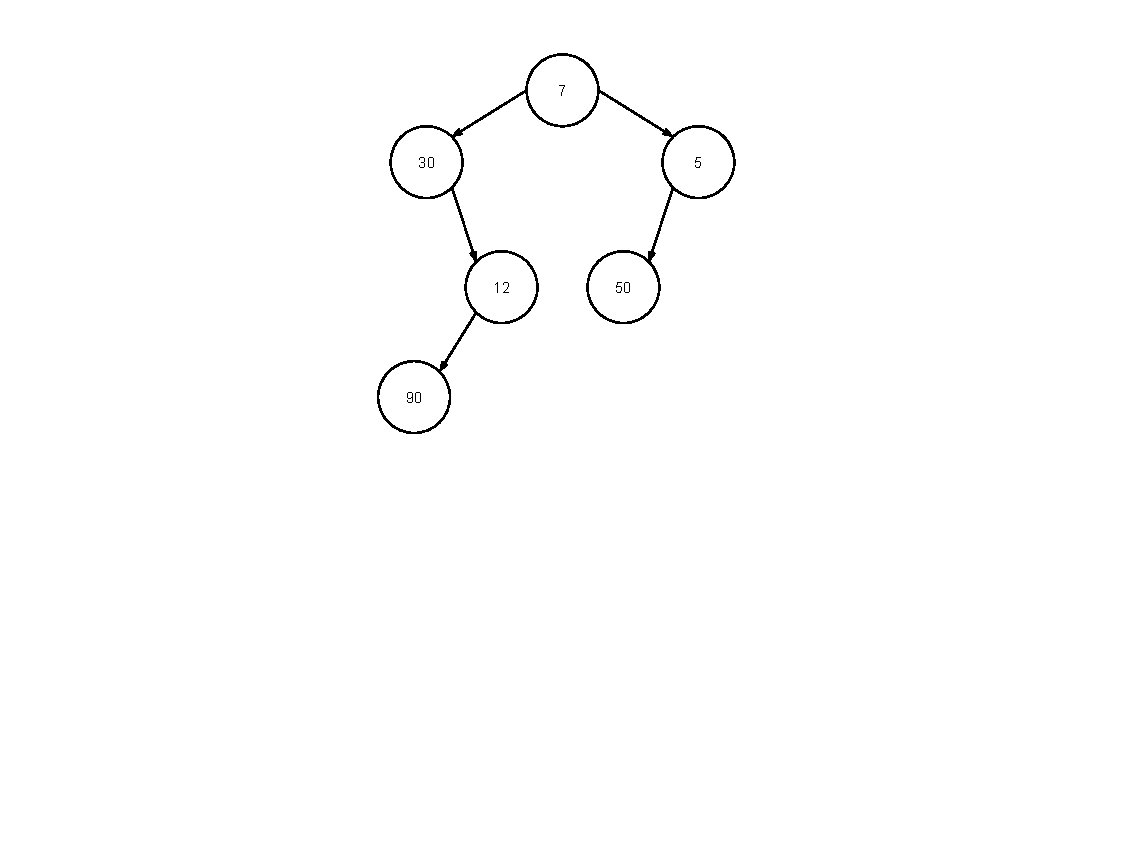
\includegraphics[width=14cm]{images/tree_arbitrary}

\end{frame}



\begin{frame}[fragile]
\frametitle{Проверка за принадлежност}

    \begin{itemize}
      \item Среща ли се елементът $y$ сред елементите на дървото $T$? 
    \end{itemize}


\begin{columns}[t]
  \begin{column}{0.65\textwidth}

    \begin{flushleft}
    \relscale{0.5}  
    \begin{itemize}
      \item Празното дърво е дърво 
      \item Ако $L_T$ и $R_T$ са дървета, а $x$ е елемент ($x \in D$), то \emph{тройката (структурата)} $T=(x,L_T,R_T)$ наричаме двоично дърво $T$ с \emph{корен} $x$, ляво поддърво $L_T$ и дясно поддърво $R_T$.
    \end{itemize}
    \end{flushleft}

  \end{column}
  \begin{column}{0.35\textwidth}

    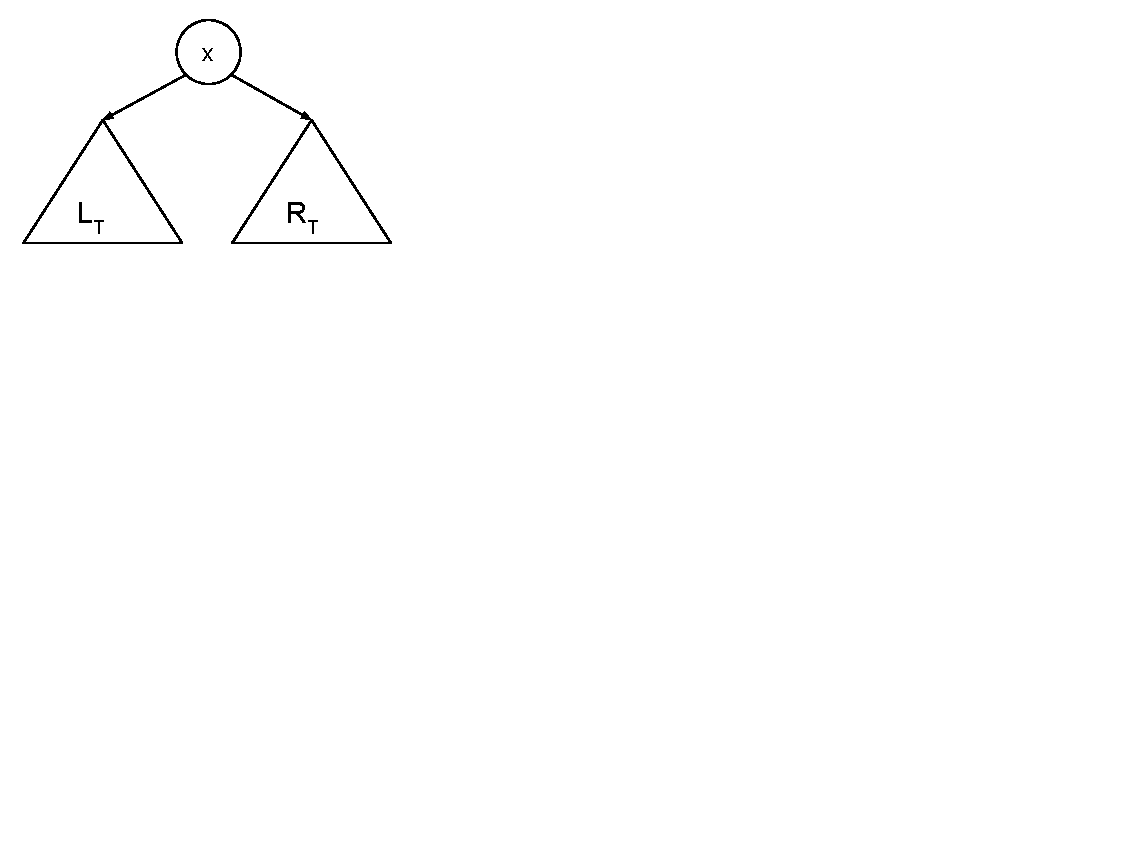
\includegraphics[width=8cm]{images/tree_recursive_op_2}

  \end{column}
\end{columns}

\vspace{-100px}

 \texttt{bool member (int y, T):}

    \begin{itemize}
      \item Ако дървото е празно, то $y$ не е елемент на дървото. \texttt{return false} 
      \item  Ако $T=(x,L_T,R_T)$ е непразно, то $y$ е елемент на $T$, ако $y==x$ или $y$ е елемент на $L_T$ или $y$ е елемент на $R_T$.
      \item \texttt{return y==root(t) || member (y, LT) || member (y,RT)} 
    \end{itemize}

\end{frame}





\begin{frame}[fragile]
\frametitle{Сума не елементите}

    \begin{itemize}
      \item Каква е сумата на елементите на дървото? 
    \end{itemize}


\begin{columns}[t]
  \begin{column}{0.65\textwidth}

    \begin{flushleft}
    \relscale{0.5}  
    \begin{itemize}
      \item Празното дърво е дърво 
      \item Ако $L_T$ и $R_T$ са дървета, а $x$ е елемент ($x \in D$), то \emph{тройката (структурата)} $T=(x,L_T,R_T)$ наричаме двоично дърво $T$ с \emph{корен} $x$, ляво поддърво $L_T$ и дясно поддърво $R_T$.
    \end{itemize}
    \end{flushleft}

  \end{column}
  \begin{column}{0.35\textwidth}

    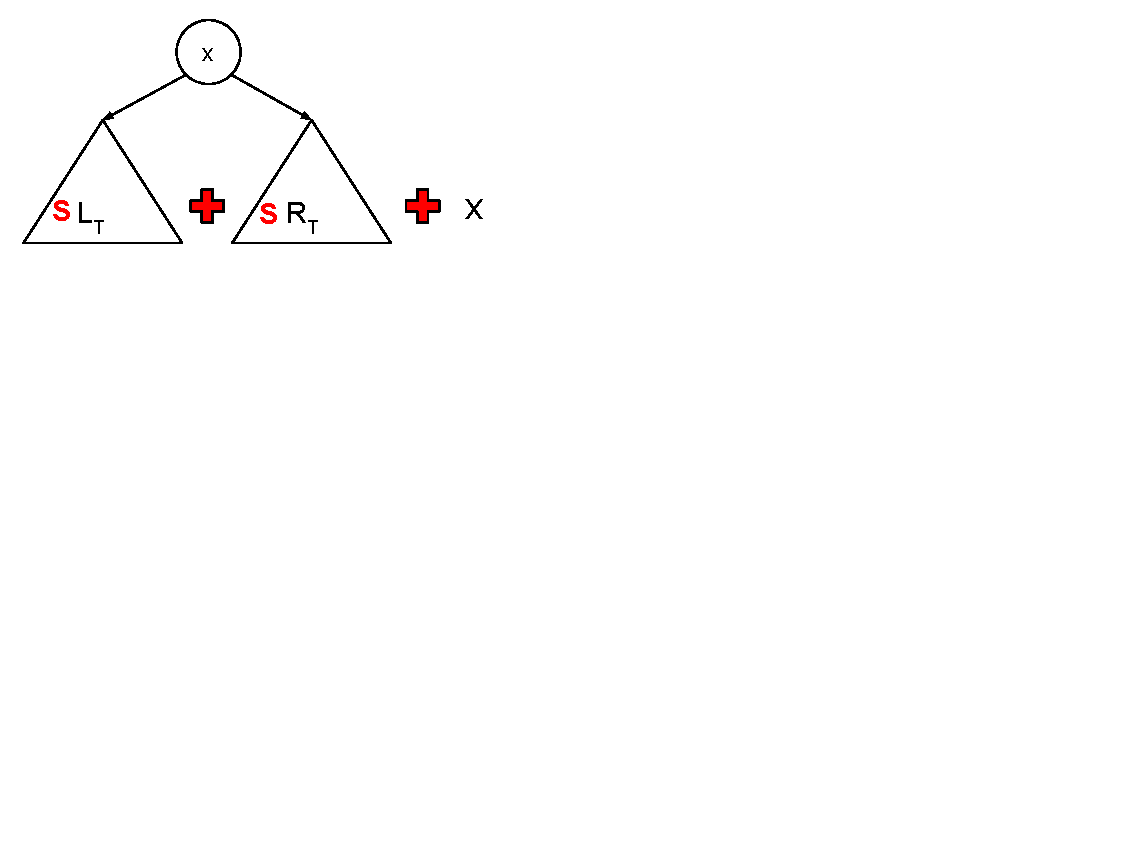
\includegraphics[width=8cm]{images/tree_recursive_op_sum}

  \end{column}
\end{columns}

\vspace{-100px}

 \texttt{int sum (T):}

    \begin{itemize}
      \item Ако дървото е празно, то сумата на елементите е $0$. \texttt{return 0} 
      \item  Ако $T=(x,L_T,R_T)$ е непразно, то сумата на елементите е сбора на сумата на елементите на $L_T$, на сумата на елементите на $R_T$ и на числото $x$.
      \item \texttt{return root(t) + sum (LT) + sum (RT)} 
    \end{itemize}

\end{frame}



\begin{frame}[fragile]
\frametitle{Други прости рекурсивни операции}

    \begin{itemize}
      \item Най-голям елемент в дървото 
      \item Брой на елементитите в дървото
      \item Височина на дървото
      \item Брой на листата в дървото
    \end{itemize}


\begin{columns}[t]
  \begin{column}{0.65\textwidth}

    \begin{flushleft}
    \relscale{0.5}  
    \begin{itemize}
      \item Празното дърво е дърво 
      \item Ако $L_T$ и $R_T$ са дървета, а $x$ е елемент ($x \in D$), то \emph{тройката (структурата)} $T=(x,L_T,R_T)$ наричаме двоично дърво $T$ с \emph{корен} $x$, ляво поддърво $L_T$ и дясно поддърво $R_T$.
    \end{itemize}
    \end{flushleft}

  \end{column}
  \begin{column}{0.35\textwidth}

    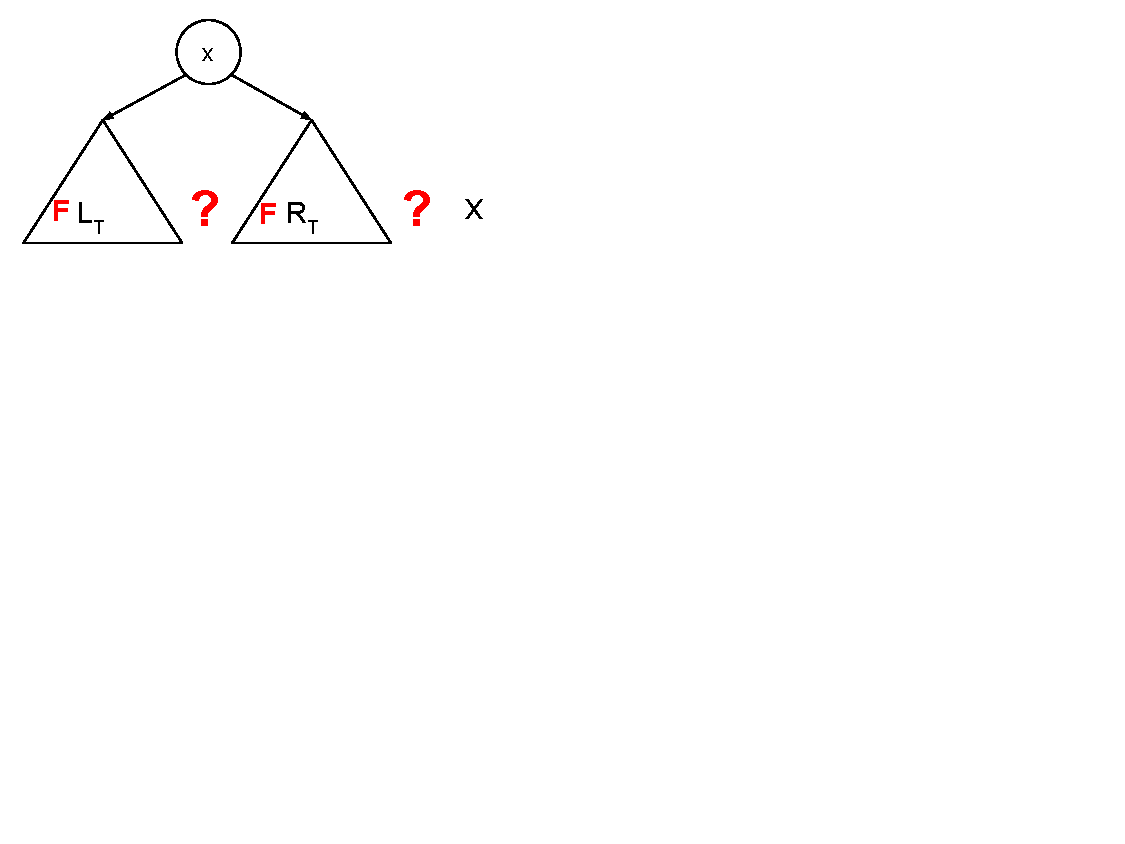
\includegraphics[width=8cm]{images/tree_recursive_op_qm}

  \end{column}
\end{columns}
\end{frame}


\begin{frame}
\begin{center}
   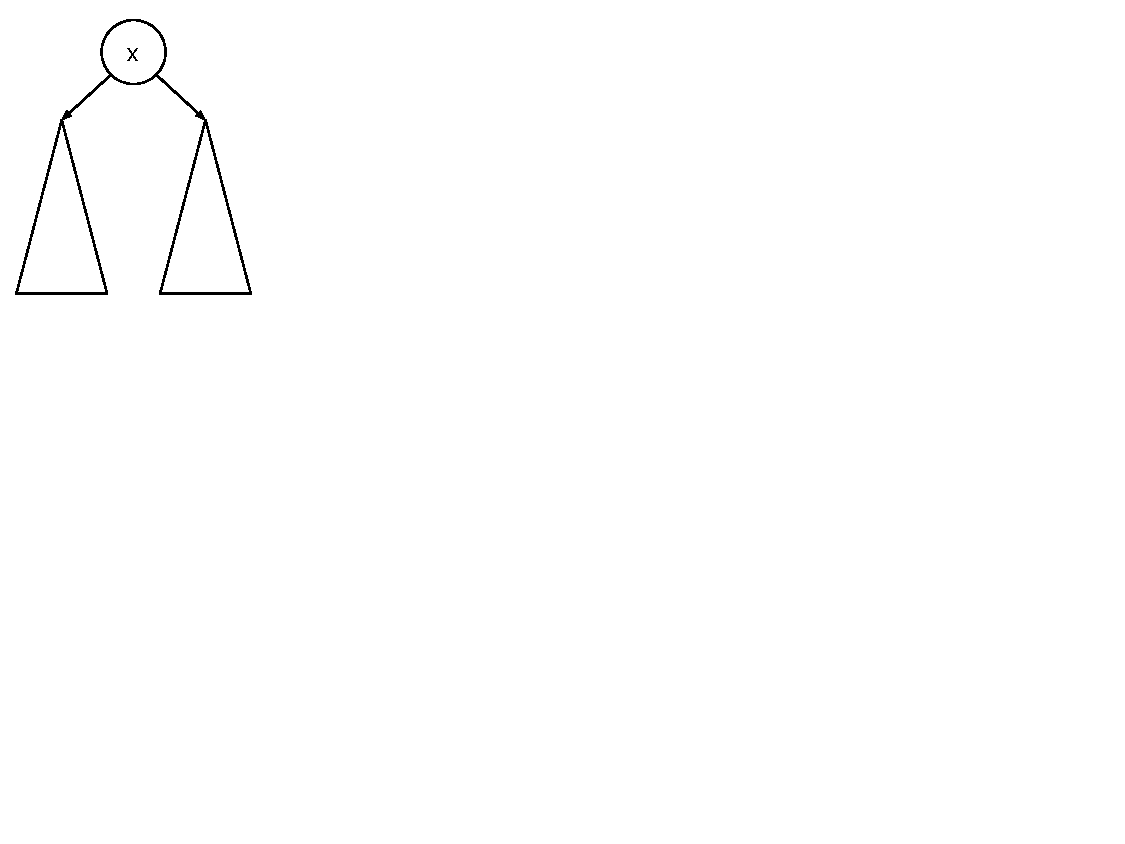
\includegraphics[width=10cm]{images/tree_recursive}
\end{center}

\vspace{-200px}
\centerline{Сериализация}
 

\end{frame} 

\section{Двоични наредени дървета} 



\begin{frame}
\centerline{Операции с двоични наредени дървета}
\end{frame}


\begin{frame}[fragile]
\frametitle{Вмъкване}

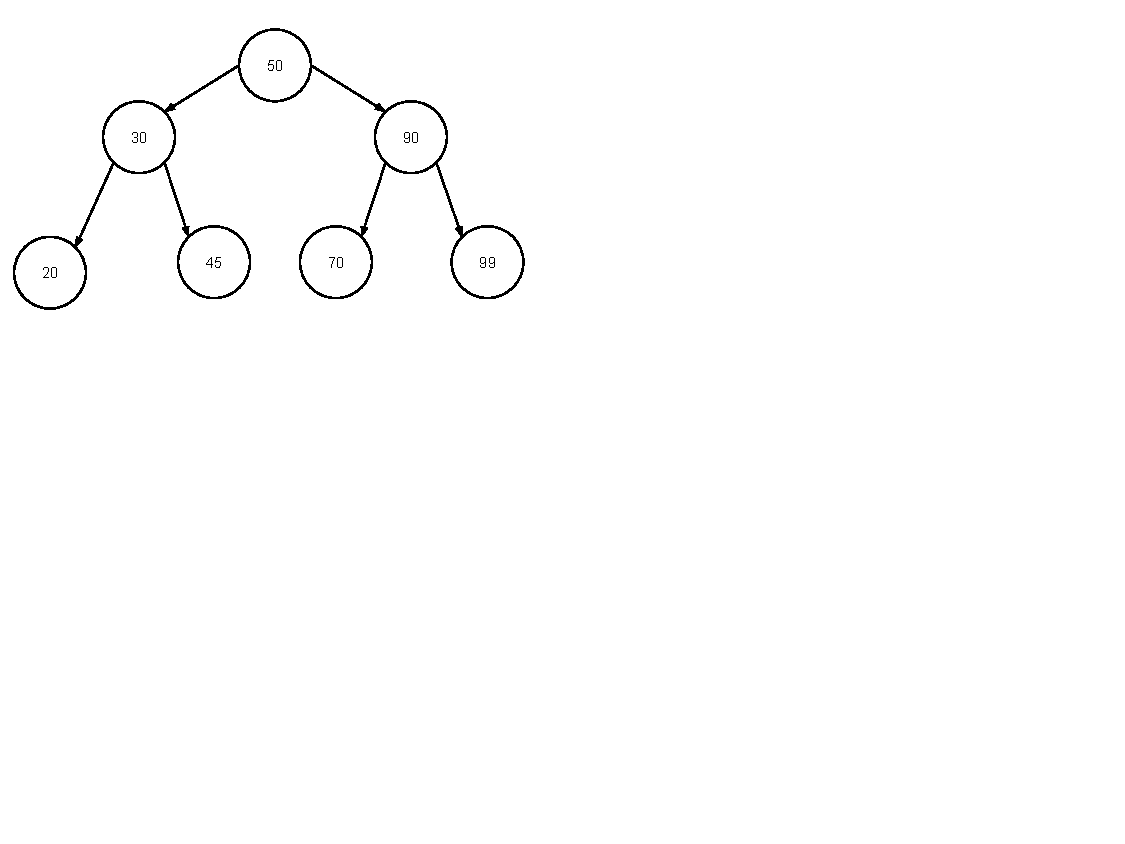
\includegraphics[width=14cm]{images/tree_bot_clean}

\end{frame}


\begin{frame}[fragile]
\frametitle{Намиране на най-голям и най-малък елемент}

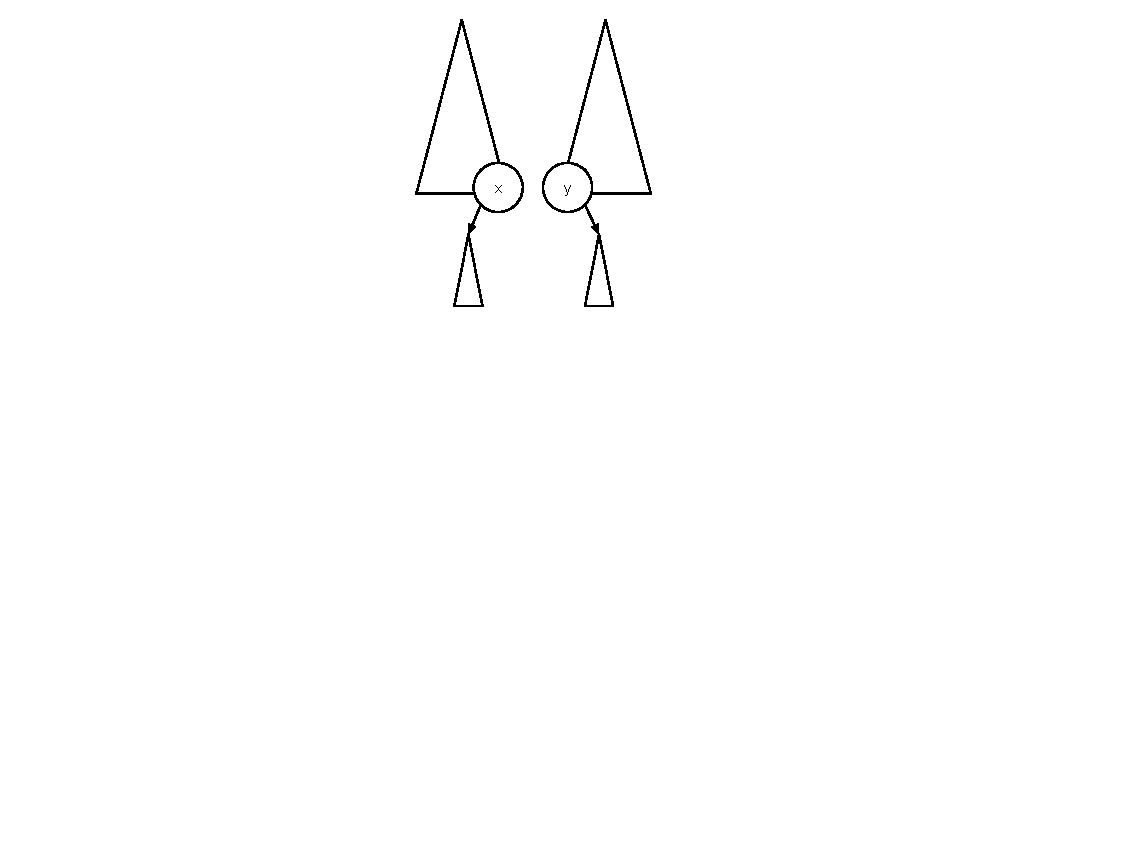
\includegraphics[width=14cm]{images/tree_extremums}

\end{frame}

\begin{frame}[fragile]
\frametitle{Изтриване}

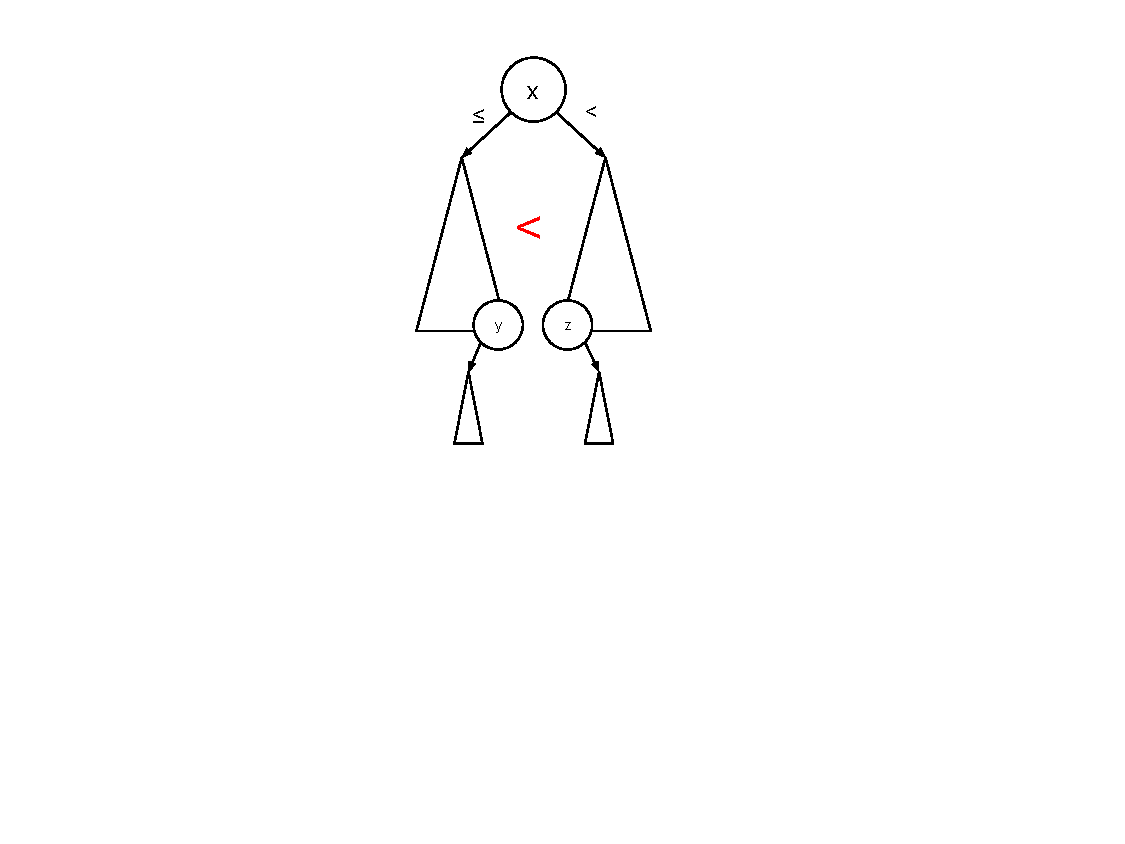
\includegraphics[width=14cm]{images/tree_delete_1}

\end{frame}



\begin{frame}[fragile]
\frametitle{Изтриване}

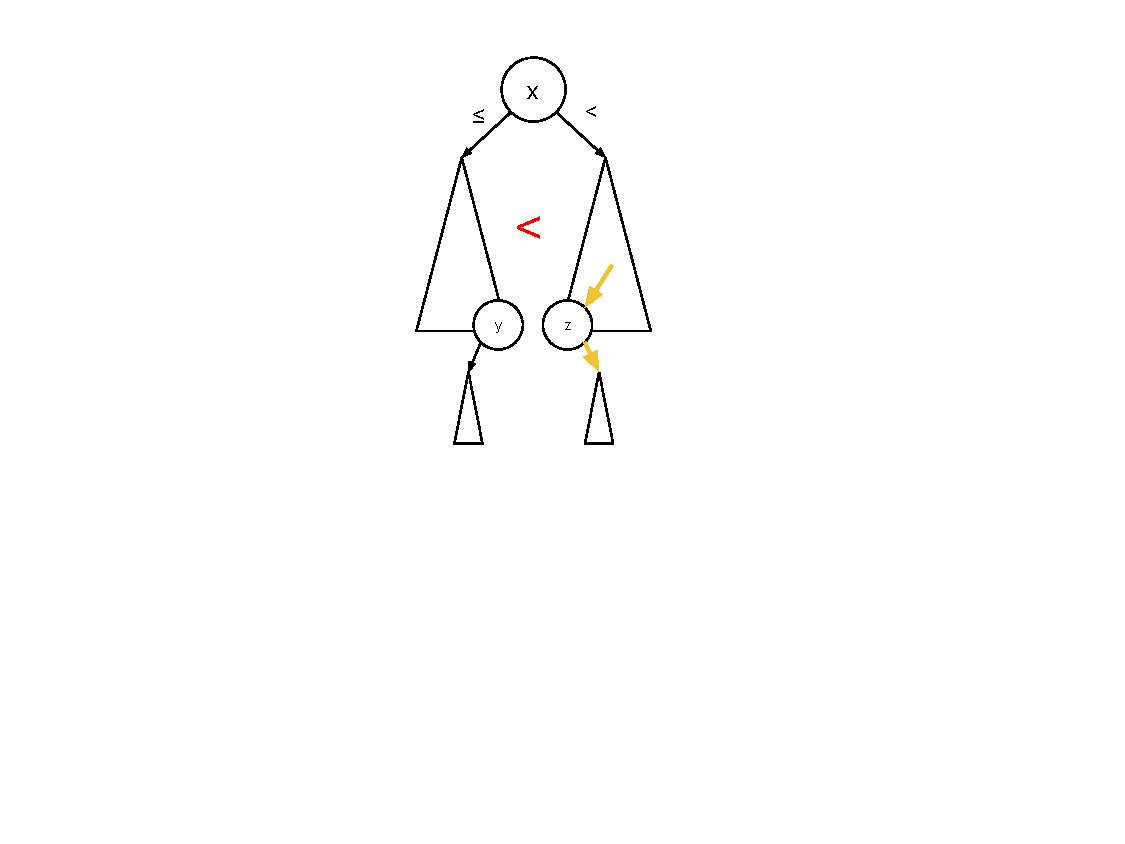
\includegraphics[width=14cm]{images/tree_delete_2}

\end{frame}


\begin{frame}[fragile]
\frametitle{Изтриване}

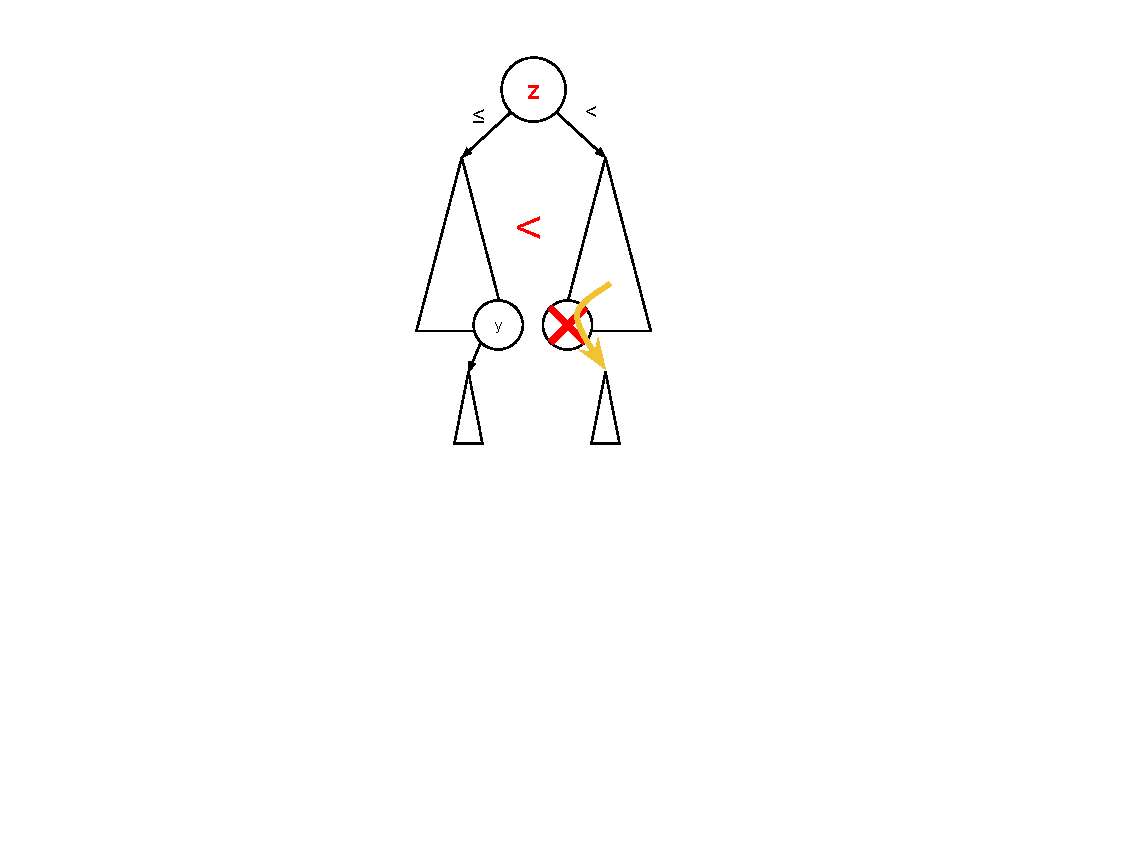
\includegraphics[width=14cm]{images/tree_delete_3}

\end{frame}

\section{Обхождания} 


\begin{frame}
\centerline{Обхождане с рекурсия VS. обхождане чрез стек}
\end{frame}


\begin{frame}[fragile]
\frametitle{Отпечатване}

\begin{itemize}
  \item Отпечатване с рекурсия 
\end{itemize}

\begin{flushleft}
  \relscale{0.7}
  \begin{lstlisting}
    void print (t){
      if (empty (t))
        return;
      print (left (t));
      cout << root (t);
      print (right (t));
    }
  \end{lstlisting}
\end{flushleft}

\end{frame}



\begin{frame}[fragile]
\frametitle{Прецес на отпечатване}



\begin{columns}[t]
  \begin{column}{0.65\textwidth}
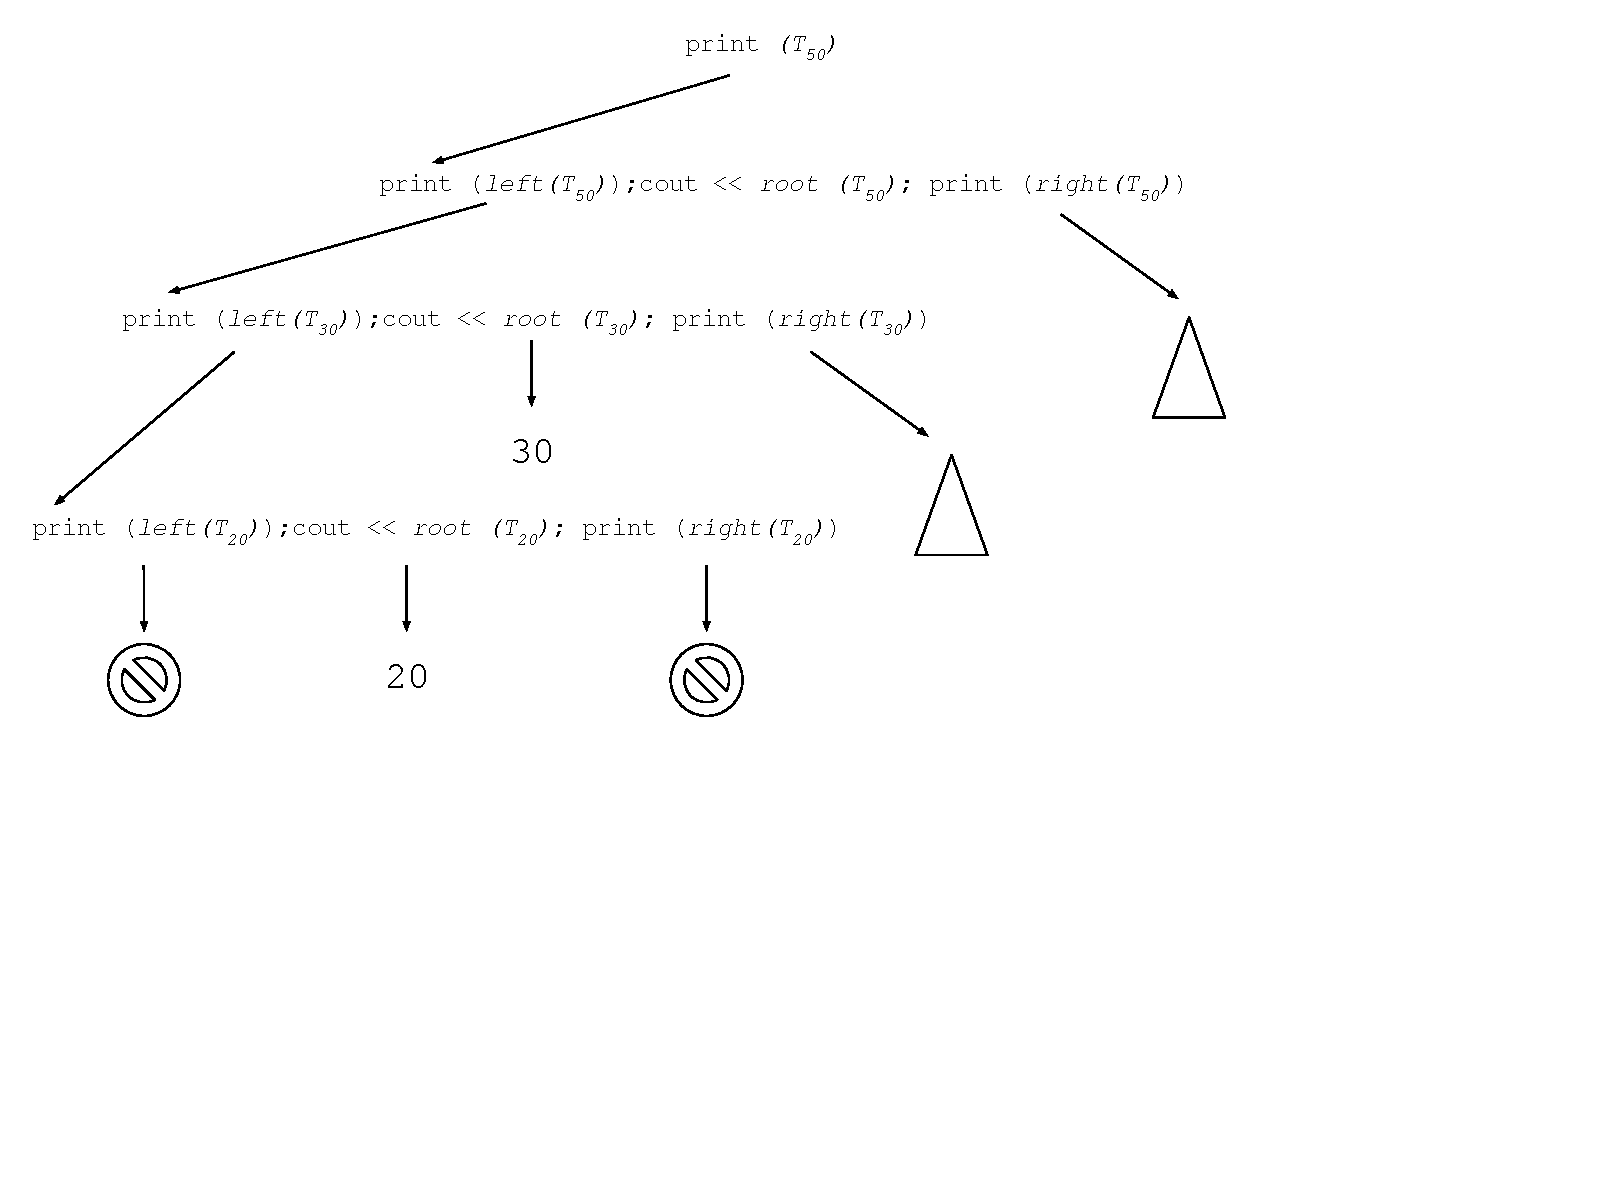
\includegraphics[width=14cm]{images/tree_print_process}
  \end{column}
  \begin{column}{0.35\textwidth}
  \vspace{-160px}
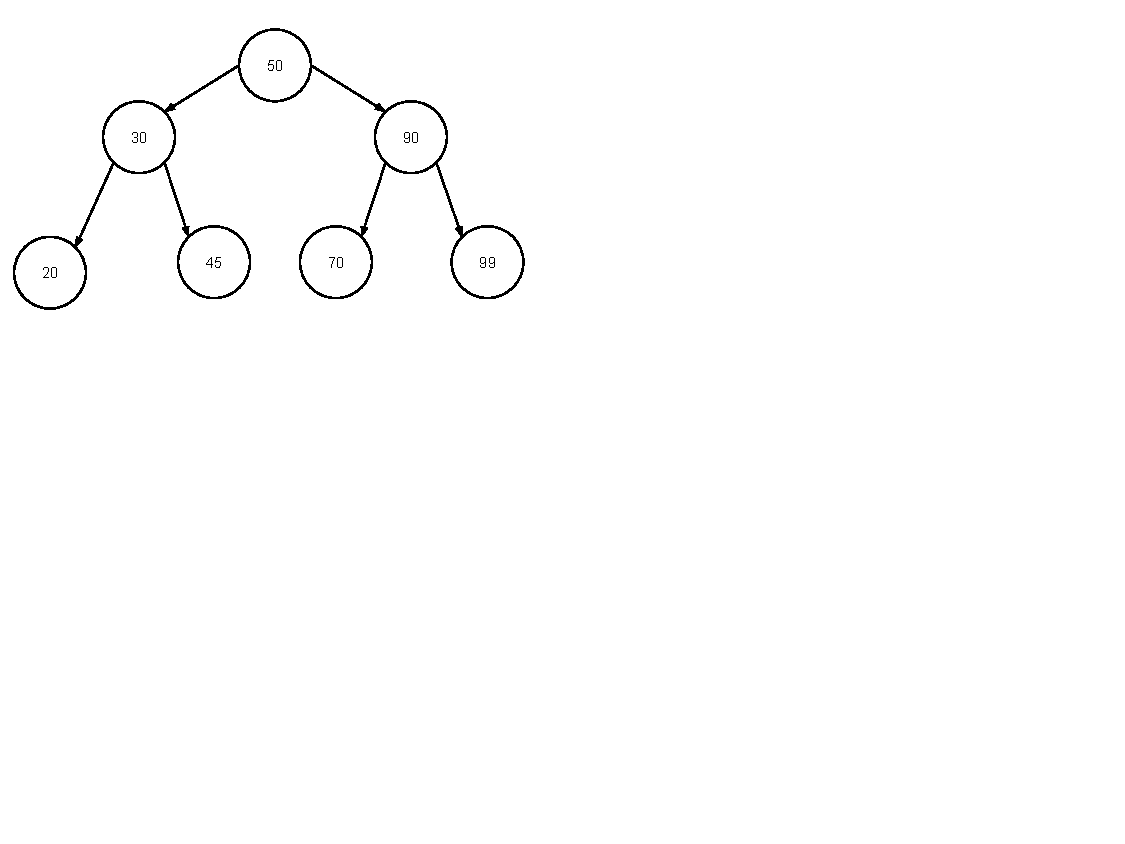
\includegraphics[width=9cm]{images/tree_bot_clean}

  \end{column}
\end{columns}
\end{frame}


\begin{frame}[fragile]
\frametitle{Прецес на отпечатване}



\begin{columns}[t]
  \begin{column}{0.65\textwidth}
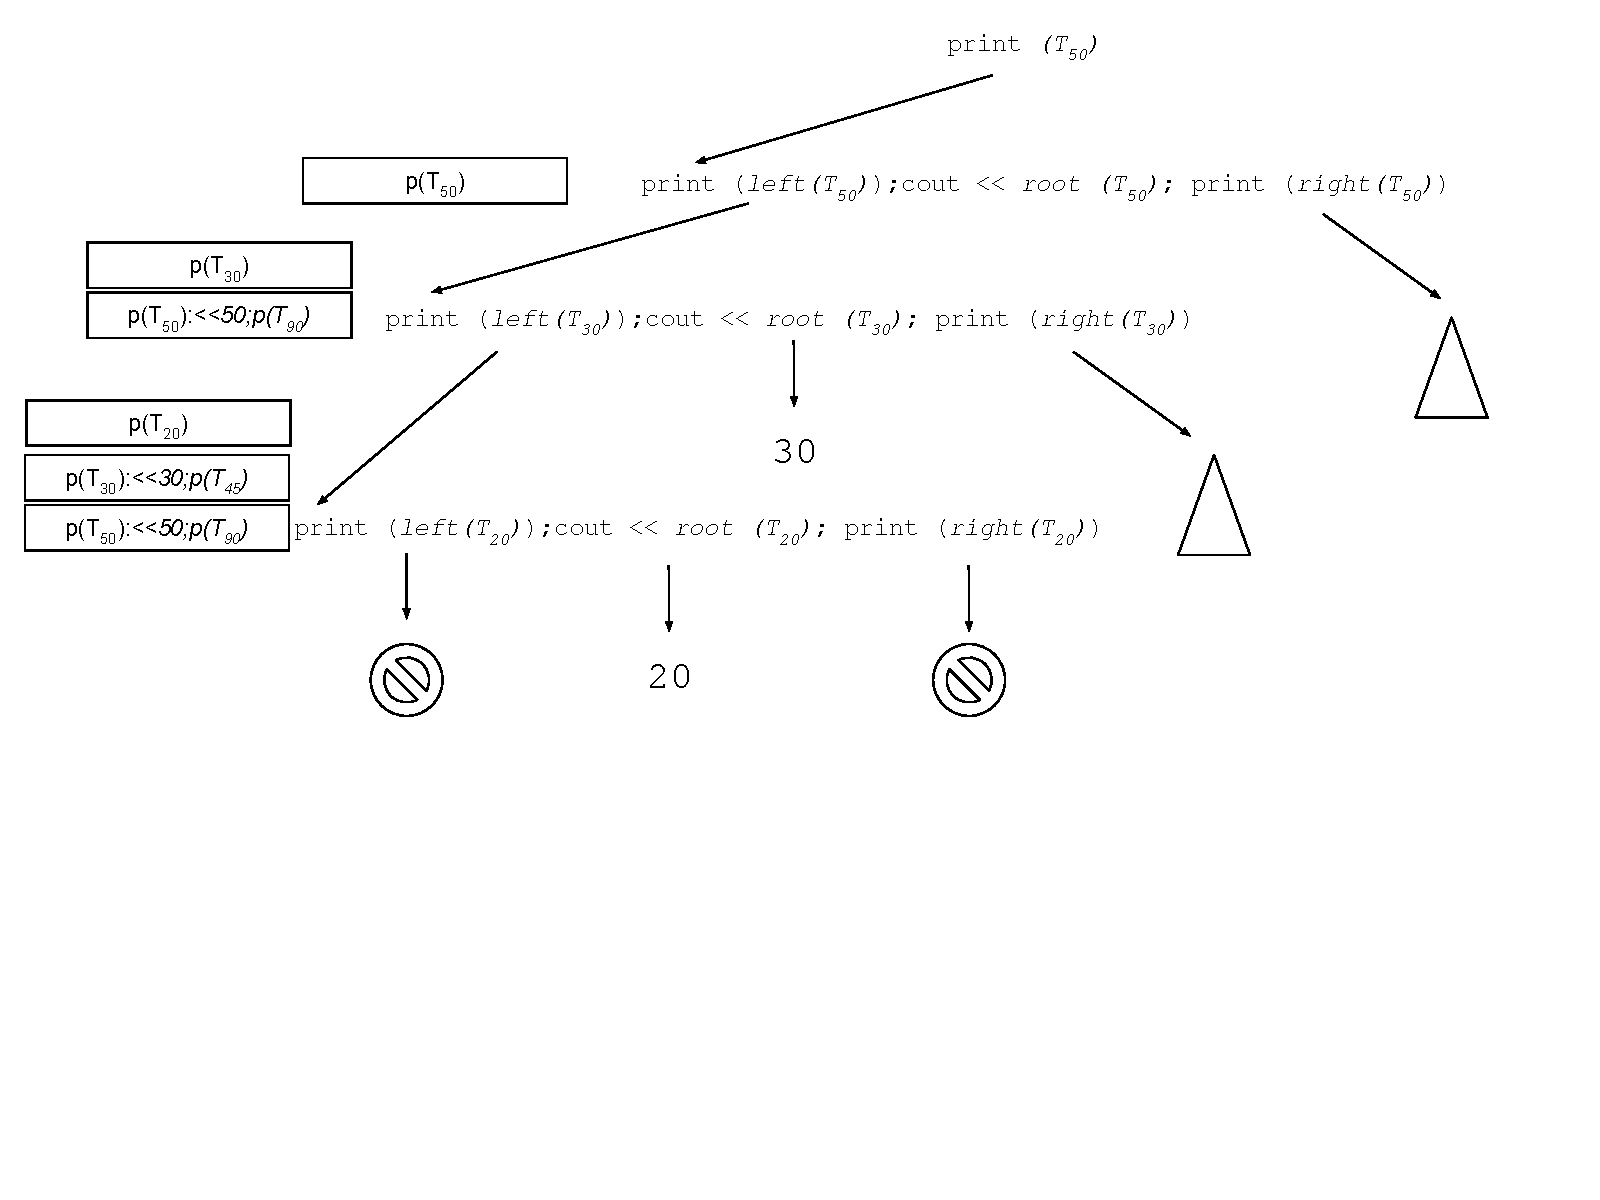
\includegraphics[width=13cm]{images/tree_print_process_stack}
  \end{column}
  \begin{column}{0.35\textwidth}
  \vspace{-140px}
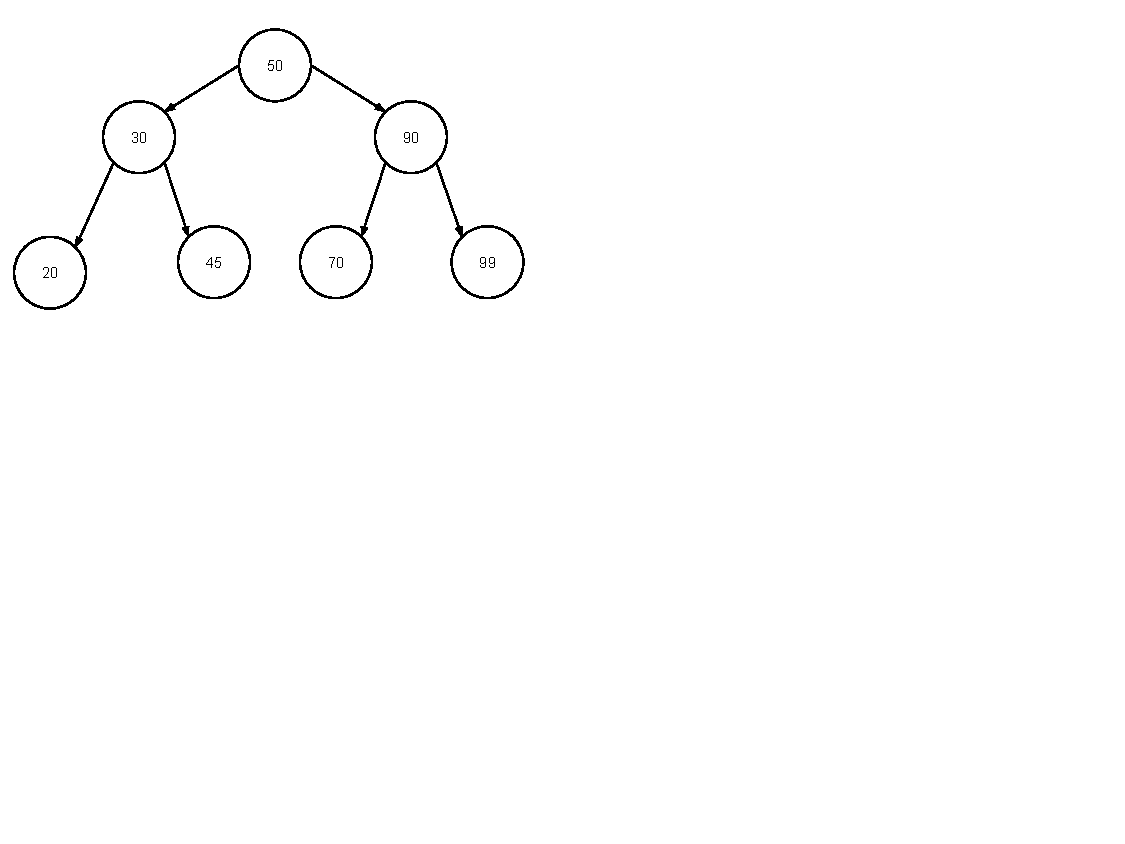
\includegraphics[width=9cm]{images/tree_bot_clean}

  \end{column}
\end{columns}
\end{frame}



\begin{frame}[fragile]
\frametitle{Отпечатване чрез стек}

\begin{itemize}
  \item Отпечатване с рекурсия 
\end{itemize}


\begin{columns}[t]
  \begin{column}{0.4\textwidth}
      \begin{flushleft}
        \relscale{0.7}
        \begin{lstlisting}
          void print (t){
            if (empty (t))
              return;
            print (left (t));
            cout << root (t);
            print (right (t));
          }
        \end{lstlisting}
      \end{flushleft}

  \end{column}
  \begin{column}{0.6\textwidth}
  
      \begin{flushleft}
        \relscale{0.7}
        \begin{lstlisting}
          void print (t){
            stack.push (t);
            while (!empty (stack)){
              x = stack.pop();
              if (x is a number) 
                 cout << x;
              else {
                stack.push (left(x)); 
                stack.push (root(x));
                stack.push (right(x));}
            }
          }
        \end{lstlisting}
      \end{flushleft}

  \end{column}
\end{columns}




\end{frame}





\begin{frame}[fragile]
\frametitle{Отпечатване чрез стек}


\begin{columns}[t]
  \begin{column}{0.4\textwidth}

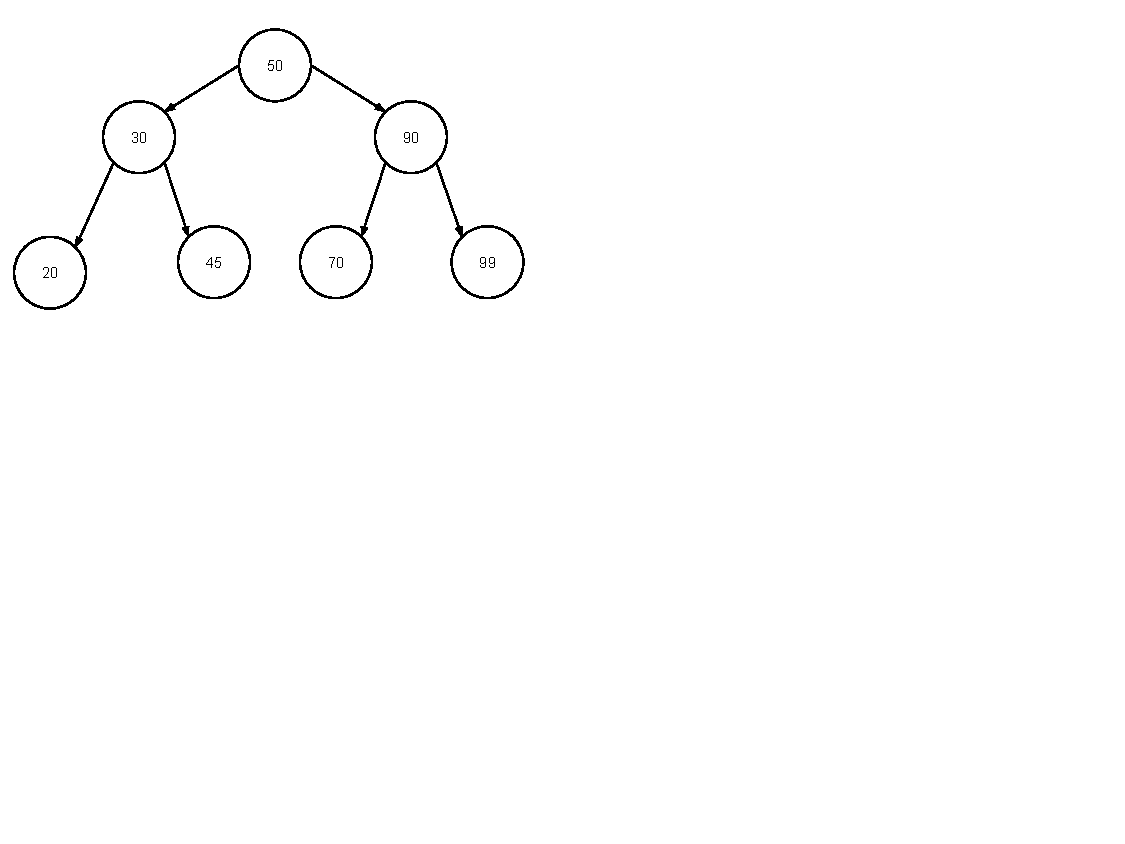
\includegraphics[width=11cm]{images/tree_bot_clean}
  \end{column}
  \begin{column}{0.6\textwidth}
  
      \begin{flushleft}
        \relscale{0.7}
        \begin{lstlisting}
          void print (t){
            stack.push (t);
            while (!empty (stack)){
              x = stack.pop();
              if (x is a number) 
                 cout << x;
              else {
                stack.push (left(x)); 
                stack.push (root(x));
                stack.push (right(x));}
            }
          }
        \end{lstlisting}
      \end{flushleft}

  \end{column}
\end{columns}

\vspace{-120px}
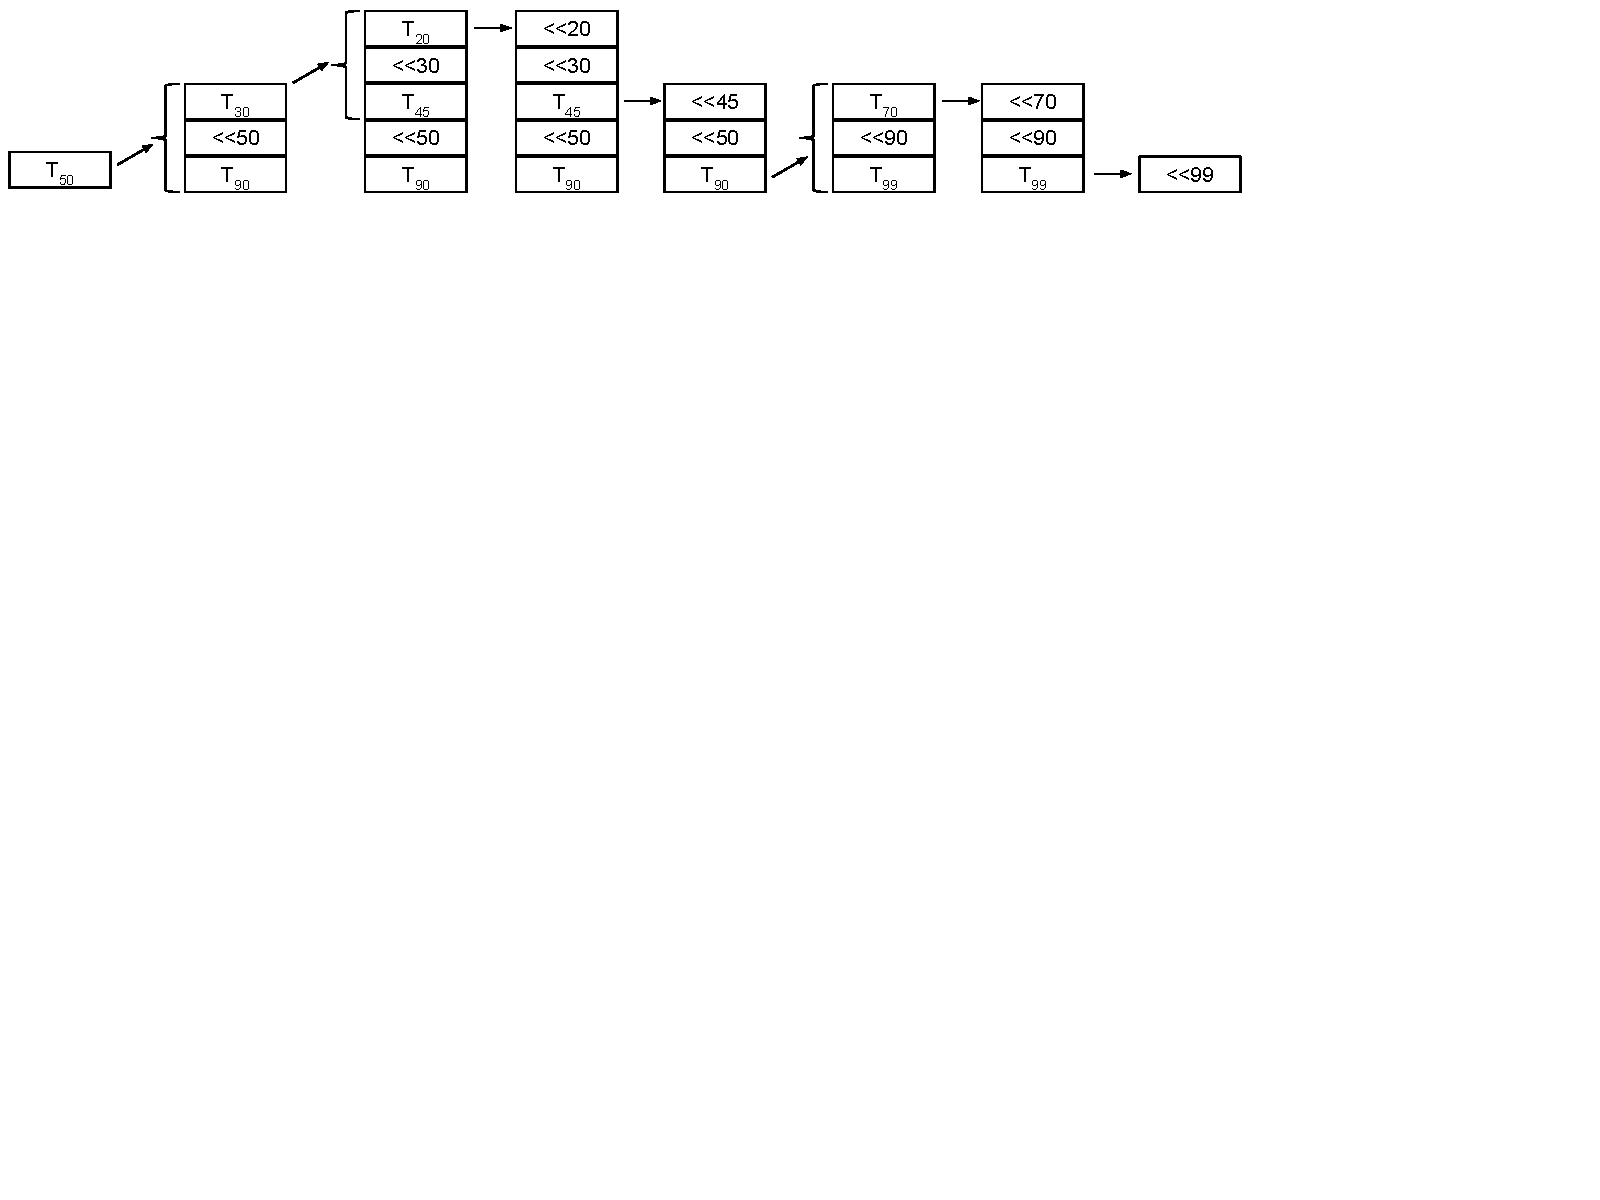
\includegraphics[width=15cm]{images/tree_print_with_stack}


\end{frame}



\begin{frame}
\centerline{Обхождане с с опашка}
\end{frame}



\begin{frame}[fragile]
\frametitle{Обхождане с опашка}

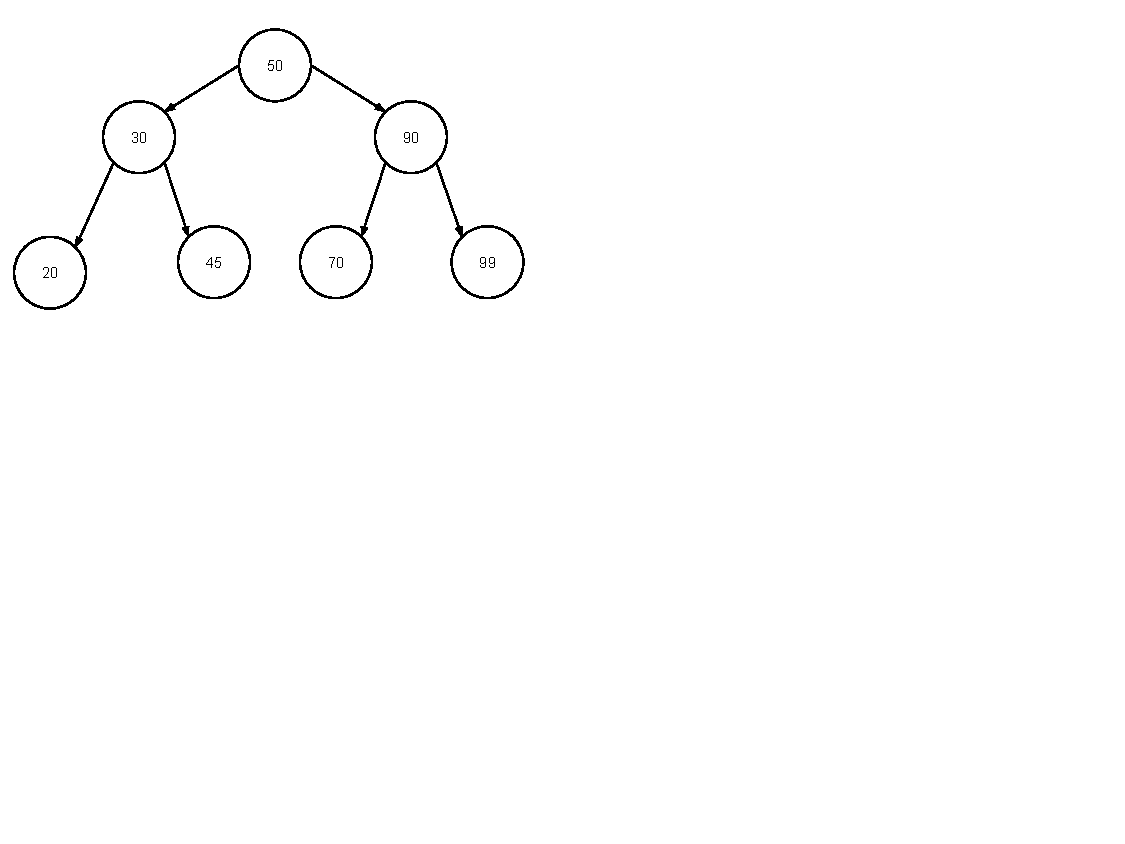
\includegraphics[width=14cm]{images/tree_bot_clean}

\end{frame}






\begin{frame}
\centerline{Въпроси?}
\end{frame}


\end{document}

\begin{columns}[t]
  \begin{column}{0.55\textwidth}

  \end{column}
  \begin{column}{0.45\textwidth}

  \end{column}
\end{columns}


